\documentclass{article}

\usepackage[preprint]{neurips_2026}
\workshoptitle{Machine Learning for Systems Workshop at NeurIPS 2026}

\usepackage[utf8]{inputenc}
\usepackage[T1]{fontenc}
\usepackage{hyperref}
\usepackage{url}
\usepackage{booktabs}
\usepackage{amsfonts}
\usepackage{microtype}
\usepackage{xcolor}
\usepackage{graphicx}
% generated by build_numbers.py from the result files; do not edit by hand
\newcommand{\aurocAdvisorRule}{0.65}
\newcommand{\aurocClock}{0.876}
\newcommand{\aurocFinal}{0.980}
\newcommand{\aurocOldAll}{0.699}
\newcommand{\aurocOldSame}{0.656}
\newcommand{\aurocPhase}{0.939}
\newcommand{\aurocVol}{0.43}
\newcommand{\awsRateMax}{150}
\newcommand{\awsRateMean}{114}
\newcommand{\awsTwoGbSeconds}{19}
\newcommand{\benchDays}{8}
\newcommand{\brierBase}{0.00147}
\newcommand{\brierFinal}{0.00136}
\newcommand{\daysBetterSixty}{98}
\newcommand{\daysBetterTen}{66}
\newcommand{\daysBetterThreeHundred}{100}
\newcommand{\diffYDHiSixty}{0.081}
\newcommand{\diffYDHiTen}{0.015}
\newcommand{\diffYDHiThreeHundred}{0.222}
\newcommand{\diffYDLoSixty}{0.054}
\newcommand{\diffYDLoTen}{-0.017}
\newcommand{\diffYDLoThreeHundred}{0.178}
\newcommand{\diffYDSixty}{0.068}
\newcommand{\diffYDTen}{0.001}
\newcommand{\diffYDThreeHundred}{0.200}
\newcommand{\drillAckBig}{34.3}
\newcommand{\drillAckSmall}{2.1}
\newcommand{\drillResumeBig}{43}
\newcommand{\drillResumeSmall}{12}
\newcommand{\events}{66}
\newcommand{\liftClock}{4.0}
\newcommand{\liftEuNorth}{42.2}
\newcommand{\liftFinal}{101.4}
\newcommand{\liftOldAll}{2.2}
\newcommand{\liftOldSame}{1.45}
\newcommand{\liftPhase}{25.5}
\newcommand{\liftSeedMax}{101.4}
\newcommand{\liftSeedMin}{98.5}
\newcommand{\nCalibPos}{6{,}787}
\newcommand{\nRegions}{8}
\newcommand{\nSeries}{768}
\newcommand{\nTestPos}{2{,}893}
\newcommand{\nTrainPos}{20{,}819}
\newcommand{\nTrainWindows}{15.9\,M}
\newcommand{\nTypes}{29}
\newcommand{\opPrecTen}{10}
\newcommand{\opPrecTwenty}{4}
\newcommand{\opRecallTen}{74}
\newcommand{\opRecallTwenty}{92}
\newcommand{\opSlowTen}{1.14}
\newcommand{\opSlowTiny}{4.01}
\newcommand{\opSlowTwenty}{1.39}
\newcommand{\ovModelSixty}{7}
\newcommand{\ovModelTen}{6}
\newcommand{\ovModelThreeHundred}{14}
\newcommand{\ovPeriodicSixty}{38}
\newcommand{\ovPeriodicTen}{36}
\newcommand{\ovPeriodicThreeHundred}{47}
\newcommand{\ovReactiveSixty}{2}
\newcommand{\ovReactiveTen}{2}
\newcommand{\ovReactiveThreeHundred}{325}
\newcommand{\ovYDSixty}{14}
\newcommand{\ovYDTen}{6}
\newcommand{\ovYDThreeHundred}{34}
\newcommand{\precNew}{9.5}
\newcommand{\precOld}{0.8}
\newcommand{\realAurocAge}{0.75}
\newcommand{\realAurocLearned}{0.77}
\newcommand{\realAurocPlace}{0.74}
\newcommand{\realAurocPrice}{0.53}
\newcommand{\realAurocPrior}{0.85}
\newcommand{\realAurocProxy}{0.50}
\newcommand{\realAurocReb}{0.66}
\newcommand{\realByPoolPlaceAge}{0.76}
\newcommand{\realByPoolPlaceAgeHi}{0.82}
\newcommand{\realByPoolPlaceAgeLo}{0.70}
\newcommand{\realCapFail}{224}
\newcommand{\realFwdPlace}{0.68}
\newcommand{\realFwdPlaceAge}{0.74}
\newcommand{\realFwdPlaceAgeHi}{0.81}
\newcommand{\realFwdPlaceAgeLo}{0.66}
\newcommand{\realFwdPlaceHi}{0.75}
\newcommand{\realFwdPlaceLo}{0.65}
\newcommand{\realHiAge}{0.80}
\newcommand{\realHiLearned}{0.83}
\newcommand{\realHiPlace}{0.80}
\newcommand{\realHiPrice}{0.60}
\newcommand{\realHiPrior}{0.89}
\newcommand{\realHiProxy}{0.51}
\newcommand{\realHiReb}{0.76}
\newcommand{\realInstances}{315}
\newcommand{\realLoAge}{0.67}
\newcommand{\realLoLearned}{0.71}
\newcommand{\realLoPlace}{0.69}
\newcommand{\realLoPrice}{0.47}
\newcommand{\realLoPrior}{0.81}
\newcommand{\realLoProxy}{0.50}
\newcommand{\realLoReb}{0.35}
\newcommand{\realMedianMin}{15}
\newcommand{\realNDays}{2}
\newcommand{\realNRegions}{4}
\newcommand{\realPlaceApSoutheast}{0.72}
\newcommand{\realPlaceEuNorth}{0.79}
\newcommand{\realPlaceUsEastOne}{0.58}
\newcommand{\realPlaceUsEastTwo}{0.59}
\newcommand{\realPosSteps}{229}
\newcommand{\realRebCovered}{7}
\newcommand{\realRebFalse}{2}
\newcommand{\realRebLead}{6}
\newcommand{\realRebUnrec}{6}
\newcommand{\realRebWarned}{7}
\newcommand{\realReclApSoutheast}{13}
\newcommand{\realReclEuNorth}{112}
\newcommand{\realReclUsEastOne}{11}
\newcommand{\realReclUsEastTwo}{16}
\newcommand{\realReclaimed}{152}
\newcommand{\realRegionPlace}{0.74}
\newcommand{\realRegionPlaceAge}{0.77}
\newcommand{\realRegionPlaceAgeHi}{0.83}
\newcommand{\realRegionPlaceAgeLo}{0.71}
\newcommand{\realRegionPlaceHi}{0.79}
\newcommand{\realRegionPlaceLo}{0.69}
\newcommand{\realSteps}{4{,}487}
\newcommand{\realTypesReclaimed}{6}
\newcommand{\realYoungAge}{0.73}
\newcommand{\realYoungLearned}{0.81}
\newcommand{\realYoungPlace}{0.81}
\newcommand{\realYoungPos}{150}
\newcommand{\realYoungPrice}{0.50}
\newcommand{\realYoungPrior}{0.88}
\newcommand{\realYoungProxy}{0.50}
\newcommand{\realYoungSteps}{1418}
\newcommand{\recallNew}{74}
\newcommand{\recallOld}{11}
\newcommand{\regDiffApSoutheast}{0.066}
\newcommand{\regDiffEuNorth}{0.200}
\newcommand{\regDiffUsEastOne}{-0.015}
\newcommand{\regDiffUsEastTwo}{0.015}
\newcommand{\regEventsApSoutheast}{22}
\newcommand{\regEventsEuNorth}{66}
\newcommand{\regEventsUsEastOne}{22}
\newcommand{\regEventsUsEastTwo}{26}
\newcommand{\regHiApSoutheast}{0.134}
\newcommand{\regHiEuNorth}{0.222}
\newcommand{\regHiUsEastOne}{0.051}
\newcommand{\regHiUsEastTwo}{0.067}
\newcommand{\regLoApSoutheast}{0.015}
\newcommand{\regLoEuNorth}{0.178}
\newcommand{\regLoUsEastOne}{-0.075}
\newcommand{\regLoUsEastTwo}{-0.057}
\newcommand{\rollAurocMax}{0.985}
\newcommand{\rollAurocMin}{0.974}
\newcommand{\rollFolds}{5}
\newcommand{\rollTrainDaysMin}{37.9}
\newcommand{\slowAdvisorYDThreeHundred}{1.60}
\newcommand{\slowModelSixty}{1.07}
\newcommand{\slowModelTen}{1.06}
\newcommand{\slowModelThreeHundred}{1.14}
\newcommand{\slowNoneSixty}{4.25}
\newcommand{\slowNoneTen}{4.25}
\newcommand{\slowNoneThreeHundred}{4.25}
\newcommand{\slowOldModelSixty}{1.91}
\newcommand{\slowOldModelTen}{1.82}
\newcommand{\slowOldModelThreeHundred}{2.48}
\newcommand{\slowOracleSixty}{1.01}
\newcommand{\slowOracleTen}{1.01}
\newcommand{\slowOracleThreeHundred}{1.03}
\newcommand{\slowPeriodicSixty}{1.38}
\newcommand{\slowPeriodicTen}{1.36}
\newcommand{\slowPeriodicThreeHundred}{1.47}
\newcommand{\slowReactiveSixty}{1.02}
\newcommand{\slowReactiveTen}{1.02}
\newcommand{\slowReactiveThreeHundred}{4.25}
\newcommand{\slowVolThreeHundred}{1.88}
\newcommand{\slowYDSixty}{1.14}
\newcommand{\slowYDTen}{1.06}
\newcommand{\slowYDThreeHundred}{1.34}
\newcommand{\synthBest}{1.29}
\newcommand{\synthLowP}{2.55}
\newcommand{\synthLowPLowR}{1.64}
\newcommand{\synthSixty}{1.34}
\newcommand{\trfAurocAdv}{0.869}
\newcommand{\trfAurocAllNineteen}{0.960}
\newcommand{\trfAurocAz}{0.876}
\newcommand{\trfAurocBase}{0.870}
\newcommand{\trfAurocCad}{0.943}
\newcommand{\trfAurocExt}{0.949}
\newcommand{\trfLiftAdv}{9.9}
\newcommand{\trfLiftAllNineteen}{50.3}
\newcommand{\trfLiftAz}{10.8}
\newcommand{\trfLiftBase}{9.8}
\newcommand{\trfLiftCad}{21.6}
\newcommand{\trfLiftExt}{35.5}
\newcommand{\trfMaxAdv}{12.3}
\newcommand{\trfMaxAllNineteen}{51.7}
\newcommand{\trfMaxAz}{12.3}
\newcommand{\trfMaxBase}{13.2}
\newcommand{\trfMaxCad}{22.5}
\newcommand{\trfMaxExt}{37.1}
\newcommand{\trfMinAdv}{7.0}
\newcommand{\trfMinAllNineteen}{48.1}
\newcommand{\trfMinAz}{9.9}
\newcommand{\trfMinBase}{7.0}
\newcommand{\trfMinCad}{20.7}
\newcommand{\trfMinExt}{32.6}
\newcommand{\xgbAurocAdv}{0.944}
\newcommand{\xgbAurocAllNineteen}{0.978}
\newcommand{\xgbAurocAllTwentyEight}{0.981}
\newcommand{\xgbAurocAz}{0.945}
\newcommand{\xgbAurocBase}{0.946}
\newcommand{\xgbAurocCad}{0.966}
\newcommand{\xgbAurocExt}{0.972}
\newcommand{\xgbLiftAdv}{14.4}
\newcommand{\xgbLiftAllNineteen}{93.2}
\newcommand{\xgbLiftAllTwentyEight}{99.3}
\newcommand{\xgbLiftAz}{15.3}
\newcommand{\xgbLiftBase}{14.8}
\newcommand{\xgbLiftCad}{26.7}
\newcommand{\xgbLiftExt}{48.5}
\newcommand{\xgbPhaseAdv}{0.806}
\newcommand{\xgbPhaseAllNineteen}{0.936}
\newcommand{\xgbPhaseAllTwentyEight}{0.941}
\newcommand{\xgbPhaseAz}{0.802}
\newcommand{\xgbPhaseBase}{0.802}
\newcommand{\xgbPhaseCad}{0.867}
\newcommand{\xgbPhaseExt}{0.920}
\newcommand{\ydSlowThreeHundred}{1.34}


\title{When Does Predicting Spot Interruptions Beat Checkpointing? A Trace-Driven Study with Real Reclaims}

\author{
  Angshuman Chakravertty\\
  SVKM's NMIMS (Deemed to be University)\\
  \texttt{angshumanchakravertty2@gmail.com}
  \And
  MD Rayyan\\
  SVKM's NMIMS (Deemed to be University)\\
  \texttt{rayyan1652@gmail.com}
}

\begin{document}
\maketitle

\begin{abstract}
Spot instances cost a fraction of on-demand capacity but can be reclaimed on two minutes' notice. We ask when predicting reclaims lets a training job do better than reacting to that notice or checkpointing on a schedule. We built Argus, a Kubernetes operator that checkpoints and migrates a job when a risk model raises an alarm, and tested it three ways. A trace-driven simulator replays real Spot price history with the model's own causal scores making the decisions. A real EKS cluster runs the whole path, and we measured in-region checkpoint upload at about \awsRateMean\,MB/s per node. A small fleet of Spot instances produced real reclaim labels. Reacting to the notice is nearly optimal while a checkpoint fits inside two minutes and fails once it does not. For 15 nodes with 300 second checkpoints, model alarms cut the extra time to finish from \ovYDThreeHundred\% (best periodic policy) to \ovModelThreeHundred\%. The catch is the label. The model predicts price spikes with AUROC \aurocFinal, but on \realPosSteps\ real reclaim steps it scores AUROC \realAurocPrice, while AWS's own placement score reaches \realAurocPlace. Prediction pays when its signal is real, and price history alone is not that signal.
\end{abstract}

\section{Introduction}
\label{sec:intro}

EC2 Spot capacity costs far less than on-demand but AWS can take it back on two minutes' notice~\citep{aws-spot}. A training job that ignores this loses everything since its last checkpoint. The loss grows with scale. If each of $N$ nodes is reclaimed with probability $p$ in an interval, the chance that at least one is reclaimed is $1-(1-p)^N$ (at $p=0.05$ and $N=16$ this is about 56\%), and a synchronous job stops when any node does. Prior systems make training itself survive preemption~\citep{varuna, bamboo, oobleck}. We ask a narrower policy question. Given a free notice and the option to checkpoint on a schedule, when is it worth predicting reclaims?

One answer is that it is never needed, because a checkpoint can simply be made fast enough to fit inside the notice. Section~\ref{sec:notice} shows where that stops being true. We measured checkpoint upload from EKS nodes to S3 at about \awsRateMean\,MB/s per node, so a model with 12 bytes of training state per parameter needs more than two minutes beyond roughly one billion parameters.

We make four contributions. First, a measured account of when the two-minute notice stops being enough (Section~\ref{sec:notice}). Second, a trace-driven benchmark in which the predictor must actually predict, with the real model's causal scores driving every decision, non-learned baselines, an alarm budget chosen on a separate slice, and intervals resampled by whole days (Sections~\ref{sec:model} and~\ref{sec:pay}). Third, real reclaim labels from CloudTrail and a test of the price-based model against them (Section~\ref{sec:real}). Fourth, a real EKS run of the full path, including three defects it exposed in our own design (Section~\ref{sec:eks}).

\section{System Design}
\label{sec:design}

Argus has three layers (Figure~\ref{fig:arch}). The prediction layer turns recent Spot price updates into a calibrated risk score and serves it at \texttt{/predict}. Training and serving share one feature module, so the model sees the same inputs in both. The orchestration layer is a \texttt{kopf} operator~\citep{k8s-operators} for a \texttt{SpotResilientJob} resource. It polls the score every minute and, when the score crosses the threshold, asks the training pod to flush a checkpoint, waits for confirmation, cordons the node and deletes the pod so it is rescheduled. The training layer is a pod that checkpoints to S3 and resumes from the latest checkpoint. A second, reactive path uses the AWS Node Termination Handler~\citep{aws-nth}, which drains the node when the real notice arrives and sends SIGTERM, and the pod's handler flushes a checkpoint.

\begin{figure}[t]
  \centering
  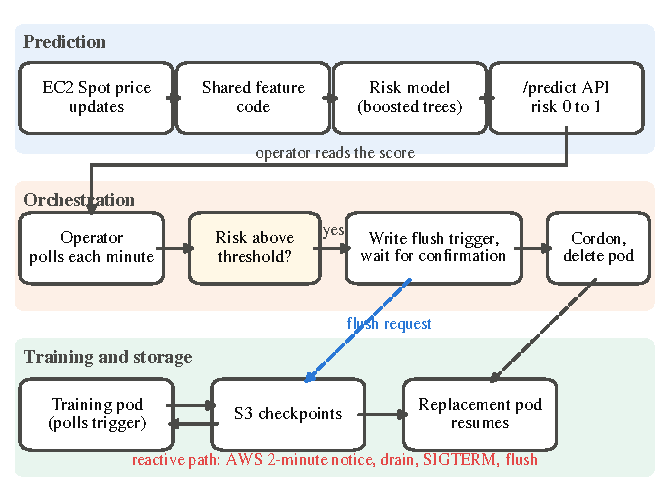
\includegraphics[width=\linewidth]{Figures/fig1_architecture.pdf}
  \caption{Argus architecture. The operator reads a risk score, asks the pod to flush, waits for an acknowledgement, and only then moves the job. The reactive path is the AWS two-minute notice.}
  \label{fig:arch}
\end{figure}

The pod role in our cluster can read and write S3 objects but cannot delete them, which shaped the handshake. The operator writes a unique request id to a trigger object. The pod saves a checkpoint, and only if the upload succeeded writes the same id to an acknowledgement object. The operator waits for its id. After a migration the operator ignores alarms for 15 minutes, the prediction horizon, because the pool's risk usually stays high after the job has left it.

\section{Evaluation}
\label{sec:eval}

\subsection{When the two-minute notice is not enough}
\label{sec:notice}

A checkpoint is useful only if it completes before the node disappears. We uploaded files of 16~MB to 2~GB from the EKS worker nodes to S3 in the same region. Rates above 500~MB were between \awsRateMean\ and \awsRateMax\,MB/s per node regardless of the number of concurrent requests, and a 2~GB file took \awsTwoGbSeconds\ seconds. Table~\ref{tab:ckpt} applies this rate to training state of 12 bytes per parameter (fp32 weights plus two Adam moments). Models of about one billion parameters already need longer than the notice, and a 7B model needs more than ten minutes, so for these jobs the free notice cannot save a checkpoint and something must act earlier.

\begin{table}[t]
  \centering
  \caption{Time to write a checkpoint from one EKS node to S3 at the measured rate. Training state is 12 bytes per parameter.}
  \label{tab:ckpt}
  \small
  \begin{tabular}{lrrrr}
\toprule
Model & Parameters & Training state & Time to S3 & Fits in 2 min? \\
\midrule
CIFAR-10 CNN (this study) & 0.3M & 4 MB & under 1 s & yes \\
ResNet-50 & 25.6M & 307 MB & 3 s & yes \\
BERT-large & 340.0M & 4.1 GB & 36 s & yes \\
1.3B-parameter LLM & 1.3B & 15.6 GB & 136 s & no \\
7B-parameter LLM & 7.0B & 84.0 GB & 735 s & no \\
\bottomrule
\end{tabular}

\end{table}

\subsection{Is the risk model a predictor?}
\label{sec:model}

The model scores whether a pool's price will rise by more than 1\% within the next 15 minutes. This is a proxy, since real reclaim labels are not public, and Section~\ref{sec:real} tests it against real reclaims. We trained on \nSeries\ price series (\nTypes\ instance types in \nRegions\ regions, 90 days) with \nTrainPos\ positive training windows, and evaluated on the last days of every series, which nothing else saw. Scaling and calibration use training and calibration slices only.

Two controls matter. AWS now publishes Spot prices about once an hour, so every price spike lands on the hour, and a rule that only knows ``the top of the hour is near'' reaches AUROC \aurocClock\ (lift \liftClock) with no model at all. The model we first shipped, trained on January to April data, scores AUROC \aurocOldAll\ (lift \liftOldAll) on the same October windows, and \aurocOldSame\ on the very instance types it was trained on. Its earlier headline lift did not survive six months. Skill must therefore be judged against the clock and among the hour-end windows where a spike is possible. The retrained gradient-boosted model reaches lift \liftFinal\ and AUROC \aurocFinal\ overall and \aurocPhase\ among hour-end windows (Figure~\ref{fig:predictor}). Across five seeds the lift ranges only from \liftSeedMin\ to \liftSeedMax. It is calibrated (Brier score \brierFinal\ against \brierBase\ for always predicting the base rate), and retraining at \rollFolds\ successive cut-off dates keeps AUROC between \rollAurocMin\ and \rollAurocMax, even with only \rollTrainDaysMin\ days of training data.

\begin{figure}[t]
  \centering
  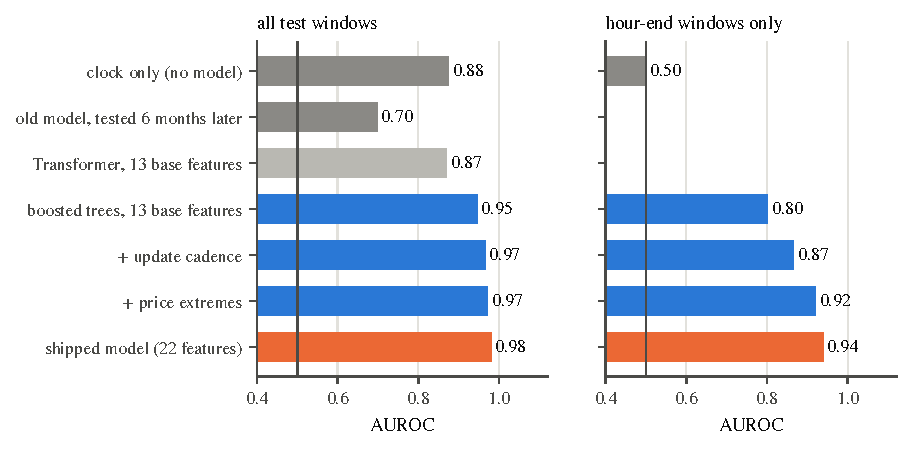
\includegraphics[width=\linewidth]{Figures/fig3_predictor.pdf}
  \caption{Test AUROC against controls. The clock-only rule is constant inside hour-end windows, so it scores 0.5 there. The old model was trained on January to April data and tested in October.}
  \label{fig:predictor}
\end{figure}

A multi-seed ablation (Appendix~\ref{app:ablation}) settles two features that earlier single runs could not. Cross-AZ price divergence and the Spot Advisor interruption rate change lift by under one point, inside the seed spread, for both boosted trees and a Transformer. What helps is how often AWS updates a price and where the price sits relative to its recent range, which raise boosted-tree lift from \xgbLiftBase\ to \xgbLiftAllNineteen. The Transformer follows the same pattern but is weaker and far less stable across seeds.

\subsection{Does prediction pay?}
\label{sec:pay}

We replay the last nine days of eu-north-1 prices for the five instance types and three AZs of our fleet. Interruptions are the price spikes in that trace (\events\ events). A synchronous job needs 12 hours of compute and is stopped by an event on any of its nodes. Checkpoints pause the job for $C$ seconds, restarts cost two minutes, and every policy is run from many start times. A policy sees only what it could see at the time. The model policy alarms when the calibrated risk of any node crosses a threshold, checkpoints and migrates. The threshold is the 10\% alarm budget chosen on the calibration slice by running the same simulation there, never on the test slice. Baselines are no protection, reacting to the notice, checkpointing every hour, checkpointing at the Young-Daly interval~\citep{young1974, daly2006} computed from the calibration slice's event rate, and an oracle with five minutes of perfect warning.

\begin{figure}[t]
  \centering
  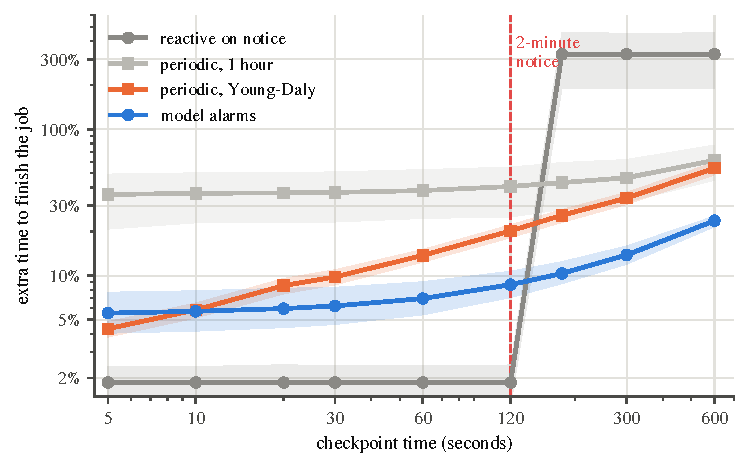
\includegraphics[width=\linewidth]{Figures/fig2_overhead_vs_checkpoint.pdf}
  \caption{Extra time to finish a 15-node job against checkpoint time. Shading is a 95\% interval resampled by whole days. Reacting to the notice is best until a checkpoint no longer fits in 120 seconds. After that, model alarms stay lowest.}
  \label{fig:main}
\end{figure}

Figure~\ref{fig:main} and Table~\ref{tab:bench} show the result. Reacting to the notice is near optimal while a checkpoint fits inside two minutes (\ovReactiveTen\% extra time) and collapses to no protection beyond it. The model matches Young-Daly for fast checkpoints and pulls ahead as checkpoints grow. At 300 seconds model alarms add \ovModelThreeHundred\% against \ovYDThreeHundred\% for Young-Daly, a difference of \diffYDThreeHundred\ in slowdown (interval \diffYDLoThreeHundred\ to \diffYDHiThreeHundred, paired and resampled by day) that favours the model on \daysBetterThreeHundred\% of the \benchDays\ days. At 60 seconds the gain is \diffYDSixty\ and at 10 seconds the two tie. The old model, at the same budget, is much worse than periodic checkpointing (slowdown \slowOldModelThreeHundred\ at 300 seconds), which shows that the model's quality is what makes prediction useful. At the budget used it catches \recallNew\% of the events with \precNew\% precision, against \recallOld\% and \precOld\% for the old model.

\begin{table}[t]
  \centering
  \caption{Slowdown against ideal (1.0 is no loss) for a 15-node job, by checkpoint time. Bold marks the best non-oracle entry where the model wins.}
  \label{tab:bench}
  \small
  \begin{tabular}{lrrr}
\toprule
Policy (15 nodes) & 10 s & 60 s & 300 s \\
\midrule
No protection & 4.25 & 4.25 & 4.25 \\
Reactive on the 2-minute notice & 1.02 & 1.02 & 4.25 \\
Periodic, every hour & 1.36 & 1.38 & 1.47 \\
Periodic, Young-Daly interval & 1.06 & 1.14 & 1.34 \\
Alarms from the old model, same budget & 1.82 & 1.91 & 2.48 \\
\textbf{Alarms from the retrained model} & 1.06 & 1.07 & \textbf{1.14} \\
Oracle, 5 minutes of perfect warning & 1.01 & 1.01 & 1.03 \\
\bottomrule
\end{tabular}

\end{table}

\paragraph{Other regions.} We repeated the replay in the seven other regions with the same protocol (Appendix~\ref{app:regions}). Among the four regions with at least 20 events the model wins in two (eu-north-1 and ap-southeast-1), ties in two (us-east-1 and us-east-2), and never loses significantly at 300 seconds. The remaining regions had one to seven events in the test slice, which is too few to separate any policies.

\subsection{Do price-based predictions anticipate real reclaims?}
\label{sec:real}

The proxy label and the simulator both treat a price spike as an interruption. To test that, we need real reclaims. AWS records a \texttt{BidEvictedEvent} in CloudTrail whenever it reclaims one of our instances~\citep{aws-cloudtrail-spot}. Our account held two such events, a c5.xlarge and an m5.large in eu-north-1b, each reclaimed minutes after launch. Neither the retrained model nor the old one raised any warning. Neither pool had a price spike.

Two events cannot support a rate, so we produced more on purpose. A fleet of tiny Spot instances, one per instance type and AZ pool, was kept alive for several hours and replaced when reclaimed, with every instance capped to self-terminate. Every five minutes we also recorded AWS's Spot placement score for each type and AZ~\citep{aws-placement}. This produced \realReclaimed\ reclaims among \realInstances\ instances. We label a pool-time step positive if a reclaim in that pool follows within 15 minutes, which gives \realPosSteps\ positive steps among \realSteps. Table~\ref{tab:real} shows how well each causal predictor ranks them.

\begin{table}[t]
  \centering
  \caption{AUROC for anticipating a real reclaim within 15 minutes, with a 95\% interval resampled by hour. The last row is not causal and asks whether the price-spike proxy coincides with real reclaims.}
  \label{tab:real}
  \small
  \begin{tabular}{lrrr}
\toprule
Predictor & AUROC & 95\% interval & First 30 min \\
\midrule
Price-history model (retrained) & 0.53 & [0.46, 0.59] & 0.50 \\
AWS Spot placement score & 0.74 & [0.69, 0.79] & 0.80 \\
AWS Rebalance Recommendation received & 0.64 & [0.43, 0.85] & 0.74 \\
Reclaim rate of the pool (leave one hour out) & 0.84 & [0.79, 0.88] & 0.86 \\
Instance age, younger is riskier (control) & 0.75 & [0.69, 0.81] & 0.74 \\
Logistic model on placement, age, price risk & 0.78 & [0.72, 0.83] & 0.83 \\
Price spike in the next 15 min (not causal) & 0.50 & [0.50, 0.51] & 0.50 \\
\bottomrule
\end{tabular}

\end{table}

The price-history model has no skill on real reclaims, and the price-spike proxy does not coincide with them. AWS's capacity signal does. This does not undo Section~\ref{sec:pay}, which is correct about what it measures, but it limits it. The benefit shown there holds if reclaims follow price spikes, and the real data says that in this region they mostly do not. A deployed system should replace or combine the price features with capacity signals such as the placement score.

\subsection{Running the full path on a real cluster}
\label{sec:eks}

We ran the operator, the retrained model served live, and training pods on a three-node EKS cluster in eu-north-1. Prices reach the service through one S3 object that a feeder refreshes, because the pod role can read only the checkpoint bucket. To trigger the predictive path on demand we set a job's threshold just below the live score. With the small CIFAR-10 model the operator saw a live score above the threshold, wrote a request, received the pod's acknowledgement after \drillAckSmall\ seconds, deleted the pod, and the replacement was ready and resumed from the checkpoint after \drillResumeSmall\ seconds. With a 2~GB checkpoint the acknowledgement took \drillAckBig\ seconds, and the replacement resumed from the full checkpoint. A second job with a high threshold ran undisturbed on another node throughout. A real node drain earlier, delivered through the Node Termination Handler, gave the same flow on the reactive path: the checkpoint reached S3 within a second of SIGTERM and the replacement pod resumed in about 75 seconds.

The cluster run found three defects in our own design that unit tests had missed. The pod role cannot delete objects, so confirming a flush by waiting for the trigger to disappear could never succeed, which led to the acknowledgement handshake. After a migration the operator re-migrated on every poll because the pool's score stayed high, so the replacement pod never stayed up, which led to the cooldown. And polling for the trigger every 100 batches made the delay depend on batch time, so with a 2~GB model the operator timed out before the pod looked, which led to polling by wall clock. A fourth, found on a first failed resume, was that a transient download error was read as ``no checkpoint'' and would have restarted training from scratch, so it now retries and then fails loudly.

\section{Limitations}
\label{sec:limits}

The strongest limit is the label. The model and the simulator use price spikes as a proxy, and Section~\ref{sec:real} shows the proxy is a poor guide to real reclaims in our data. The real-label test covers one region, tiny instances, and a few hours, and sensors that are reclaimed within minutes of launch may behave differently from long-running training nodes. The benchmark covers nine days per region and the intervals, though resampled by day, rest on that short record. The simulator assumes the notice always arrives, that a migrated node cannot be reclaimed for 15 minutes, and that a synchronous job is stopped by any node. The operator manages jobs individually and does not itself coordinate the nodes of one synchronous job. Checkpoint cost is a parameter, tied to model size through the measured S3 rate, not measured for each model. The live price sources that call the EC2 API need an IAM permission we could not grant, so the cluster run used an S3 feed.

\section{Related Work and Conclusion}
\label{sec:related}

Varuna, Bamboo and Oobleck make training survive preemption through elastic rescaling, redundant computation or pipeline templates~\citep{varuna, bamboo, oobleck}. CheckFreq and Gemini make checkpoints cheaper or faster~\citep{checkfreq, gemini}. The optimal periodic interval is classical~\citep{young1974, daly2006}, and we use it as the strongest non-learned baseline. Learned failure and interruption prediction for systems~\citep{node-failure-pred} is the closest line of work, and our contribution is to test such a predictor against real events.

Reacting to the notice is enough while checkpoints fit inside it. Once they do not, which happens for models beyond about a billion parameters, a good predictor can beat the best periodic policy by a wide margin. Our predictor is good at price spikes and not at real reclaims, while AWS's placement score looks promising. The next step is training on real reclaim labels with capacity features, and the sensor fleet and label pipeline in the released code are a start.

\bibliographystyle{plainnat}
\bibliography{references}

\appendix

\section{Feature ablation}
\label{app:ablation}

\begin{table}[h]
  \centering
  \caption{Test lift and AUROC by feature set, mean of three seeds. Hour-end AUROC is measured among the windows where a spike is possible.}
  \small
  \begin{tabular}{lrrrrr}
\toprule
& \multicolumn{3}{c}{Boosted trees} & \multicolumn{2}{c}{Transformer} \\
\cmidrule(lr){2-4}\cmidrule(lr){5-6}
Features & Lift & AUROC & Hour-end AUROC & Lift & AUROC \\
\midrule
13 base features & 14.8 & 0.946 & 0.802 & 9.8 & 0.870 \\
+ cross-AZ price divergence & 15.3 & 0.945 & 0.802 & 10.8 & 0.876 \\
+ Spot Advisor interruption rate & 14.4 & 0.944 & 0.806 & 9.9 & 0.869 \\
+ update cadence & 26.7 & 0.966 & 0.867 & 21.6 & 0.943 \\
+ price extremes & 48.5 & 0.972 & 0.920 & 35.5 & 0.949 \\
all 19 features & 93.2 & 0.978 & 0.936 & 50.3 & 0.960 \\
all 28 features & 99.3 & 0.981 & 0.941 & &  \\
\bottomrule
\end{tabular}

\end{table}

\section{Rolling-origin evaluation}
\label{app:rolling}

\begin{table}[h]
  \centering
  \caption{The model retrained from scratch at five cut-off dates and tested on each following nine-day block.}
  \small
  \begin{tabular}{lrrrrr}
\toprule
Test block & Train days & Positives & Lift & AUROC & Hour-end AUROC \\
\midrule
10-04 to 10-13 & 74 & 2{,}947 & 98.6 & 0.978 & 0.938 \\
09-25 to 10-04 & 65 & 6{,}883 & 68.1 & 0.982 & 0.948 \\
09-16 to 09-25 & 56 & 1{,}621 & 127.8 & 0.977 & 0.936 \\
09-07 to 09-16 & 47 & 2{,}549 & 104.8 & 0.985 & 0.948 \\
08-29 to 09-07 & 38 & 3{,}025 & 67.6 & 0.974 & 0.925 \\
\bottomrule
\end{tabular}

\end{table}

\section{Other regions}
\label{app:regions}

\begin{table}[h]
  \centering
  \caption{15-node jobs with 300 second checkpoints. Difference is the slowdown removed relative to Young-Daly, so positive favours the model. Intervals resample whole days.}
  \small
  \begin{tabular}{lrrrrl}
\toprule
Region & Events & Model & Young-Daly & Difference [95\% interval] & Read \\
\midrule
eu-north-1 & 66 & 1.14 & 1.34 & +0.200 [+0.178, +0.222] & model better \\
us-east-2 & 26 & 1.16 & 1.17 & +0.015 [-0.057, +0.067] & tie \\
ap-southeast-1 & 22 & 1.10 & 1.16 & +0.066 [+0.015, +0.134] & model better \\
us-east-1 & 22 & 1.15 & 1.13 & -0.015 [-0.075, +0.051] & tie \\
us-west-2 & 7 & 1.06 & 1.07 & +0.009 [-0.014, +0.035] & too few events \\
eu-central-1 & 3 & 1.06 & 1.06 & +0.000 [-0.061, +0.064] & too few events \\
eu-west-1 & 1 & 1.02 & 1.03 & +0.005 [-0.006, +0.017] & too few events \\
ap-south-1 & 1 & 1.01 & 1.15 & +0.137 [+0.130, +0.144] & too few events \\
\bottomrule
\end{tabular}

\end{table}

\begin{figure}[h]
  \centering
  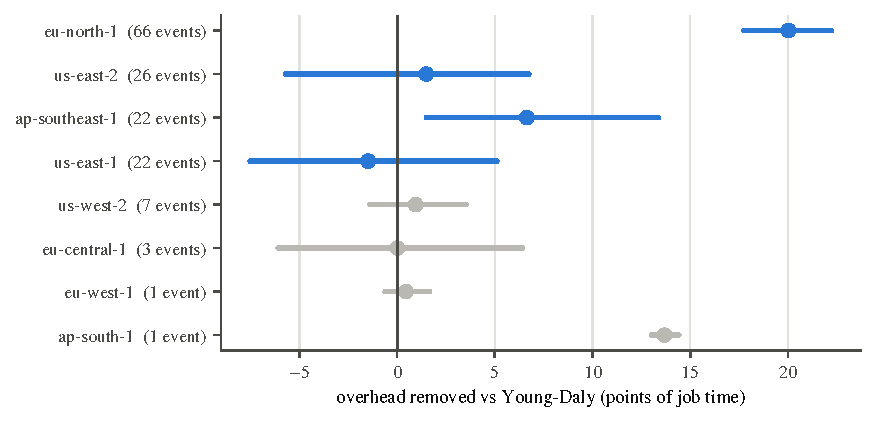
\includegraphics[width=\linewidth]{Figures/fig4_regions.pdf}
  \caption{Overhead removed relative to Young-Daly by region. Grey marks regions with fewer than 20 events.}
\end{figure}

\section{Reproducibility}

All numbers in this paper are generated from the result files by \texttt{Paper/v2/build\_numbers.py} and \texttt{build\_tables.py}. Code, data pipeline, simulator, cluster manifests and the sensor fleet are in the project repository.

\end{document}
